\appendix{Specyfikacja akcji}\label{appendix:6}

Specyfikacja w formie elektronicznej znajduje się pod linkiem: \url{https://github.com/0x41gawor/lupus/blob/master/docs/spec/actions.md}.

Specyfikacja \hyperlink{def:akcja}{\textbf{Akcji}} w \hyperlink{def:lupn}{\textbf{LupN}} znajduje się w \hyperref[appendix:3]{Załączniku 3}. Niniejszy dokument prezentuje przykładowe działanie \hyperlink{def:akcja}{\textbf{Akcji}} na \hyperlink{def:dane}{\textbf{Danych}}.

\hyperlink{def:akcja}{\textbf{Akcje}} zostały opracowane jako najbardziej atomowe operacje, które, gdy zostaną odpowiednio połączone, stanowią narzędzie umożliwiające \hyperlink{def:projektant}{\textbf{Projektantowi Pętli}} pełne operowanie na \hyperlink{def:dane}{\textbf{Danych}}.

Czasami operacja, która na pierwszy rzut oka wydaje się atomowa, wymaga użycia dwóch połączonych \hyperlink{def:akcja}{\textbf{Akcji}}. Z drugiej strony, zdarza się, że operacja początkowo uznana za atomową okazuje się jedynie szczególnym przypadkiem bardziej ogólnej operacji. Dobrym przykładem jest nieistniejąca już \hyperlink{def:akcja}{\textbf{Akcja}} \texttt{concat}. Została ona zaprojektowana do łączenia dwóch pól w jedno, jednak okazało się, że jest to specyficzny przypadek \hyperlink{def:akcja}{\textbf{Akcji}} \texttt{nest}, w której lista \texttt{InputKey} zawiera tylko dwa elementy.

\subsection{Podział ogólny}

Mamy 8 typów akcji:

\begin{itemize}
    \item \textbf{Send}
    \item \textbf{Nest}
    \item \textbf{Remove}
    \item \textbf{Rename}
    \item \textbf{Duplicate}
    \item \textbf{Insert}
    \item \textbf{Print}
    \item \textbf{Switch}
\end{itemize}

Możemy wyróżnić następujące kategorie:

\begin{itemize}
    \item 6 akcji, które mogą być używane do modyfikacji danych: \\ 
          \texttt{\{Send, Nest, Remove, Rename, Duplicate, Insert\}}
    \item 1 akcja do komunikacji z \textbf{Elementami Zewnętrznymi}: \\ 
          \texttt{\{Send\}}
    \item 2 akcje do debugowania: \\ 
          \texttt{\{Insert, Print\}}
    \item 1 akcja do logowania: \\ 
          \texttt{\{Print\}}
    \item 1 akcja do sterowania przepływem \textbf{workflow akcji}: \\ 
          \texttt{\{Switch\}}
\end{itemize}

\subsection{Przykłady}

Ta sekcja przedstawi przykładowe użycie 6 akcji, które mogą modyfikować dane.

Każdy przykład zawiera:

\begin{itemize}
    \item reprezentację JSON stanu \textbf{danych} przed modyfikacją akcji,
    \item notację \textbf{LupN} zastosowanej akcji,
    \item reprezentację JSON stanu \textbf{danych} po modyfikacji akcji
\end{itemize}

\subsubsection{Send}
\begin{figure}[!h]
    \centering 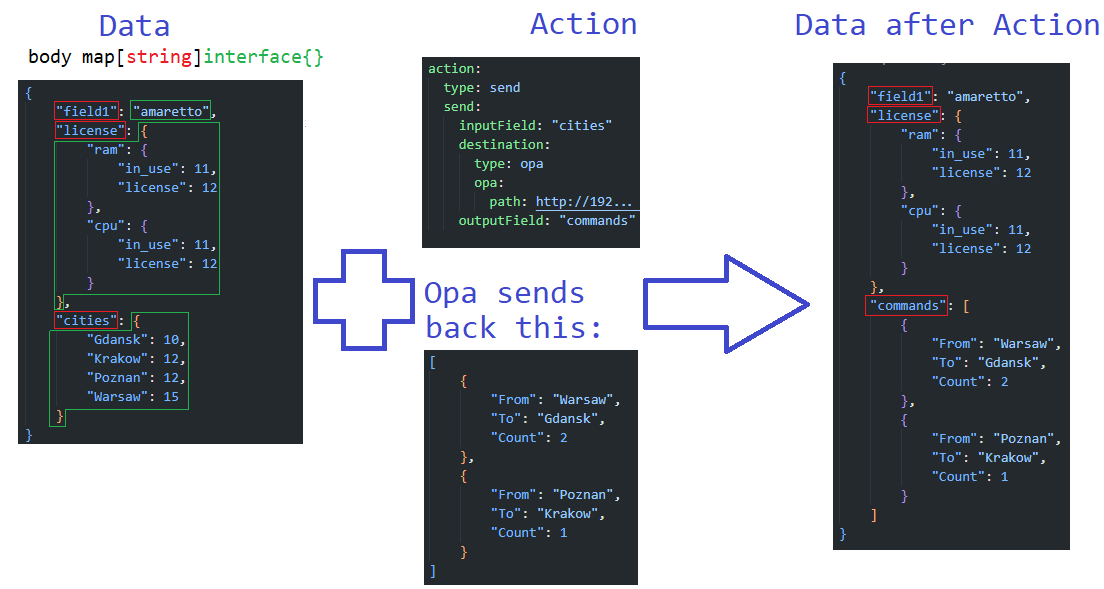
\includegraphics[width=1\linewidth]{a6-send.png}
    \caption{Przykład modyfikacji danych przez akcje Send}\label{fig:a6-send}
\end{figure}
\subsubsection{Nest}
\begin{figure}[!h]
    \centering 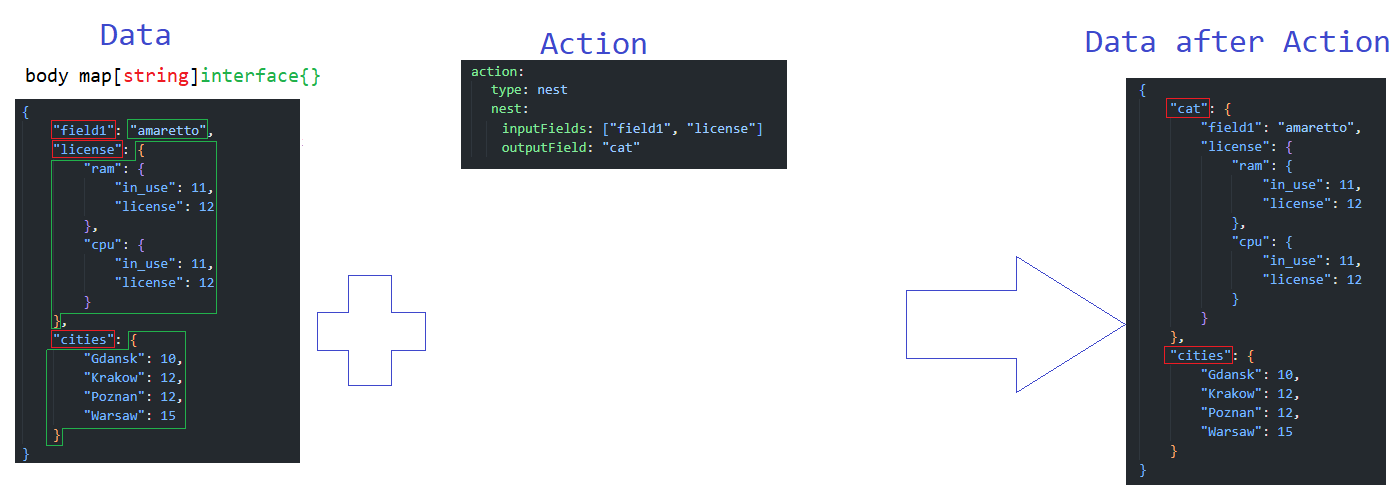
\includegraphics[width=1\linewidth]{a6-nest.png}
    \caption{Przykład modyfikacji danych przez akcje Nest}\label{fig:a6-nest}
\end{figure}
\subsubsection{Remove}
\begin{figure}[!h]
    \centering 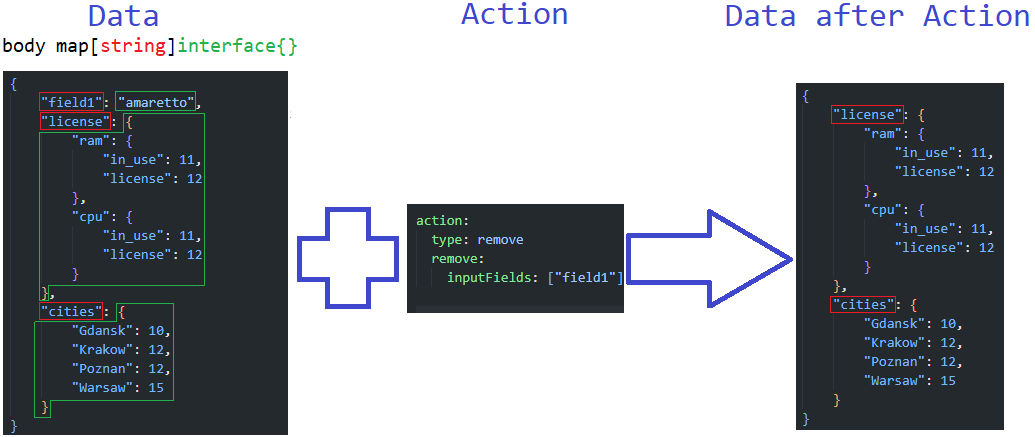
\includegraphics[width=1\linewidth]{a6-remove.png}
    \caption{Przykład modyfikacji danych przez akcje Remove}\label{fig:a6-remove}
\end{figure}
\subsubsection{Rename}
\begin{figure}[!h]
    \centering 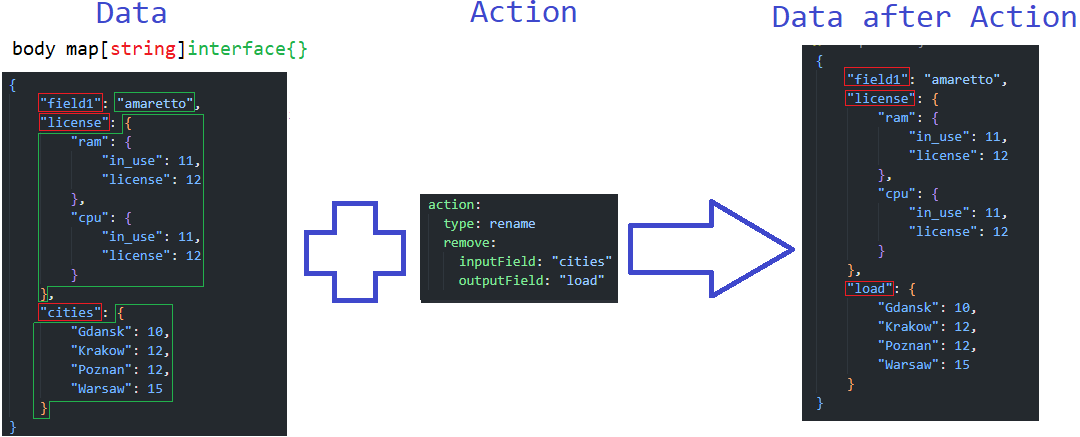
\includegraphics[width=1\linewidth]{a6-rename.png}
    \caption{Przykład modyfikacji danych przez akcje Rename}\label{fig:a6-rename}
\end{figure}
\subsubsection{Duplicate}
\begin{figure}[!h]
    \centering 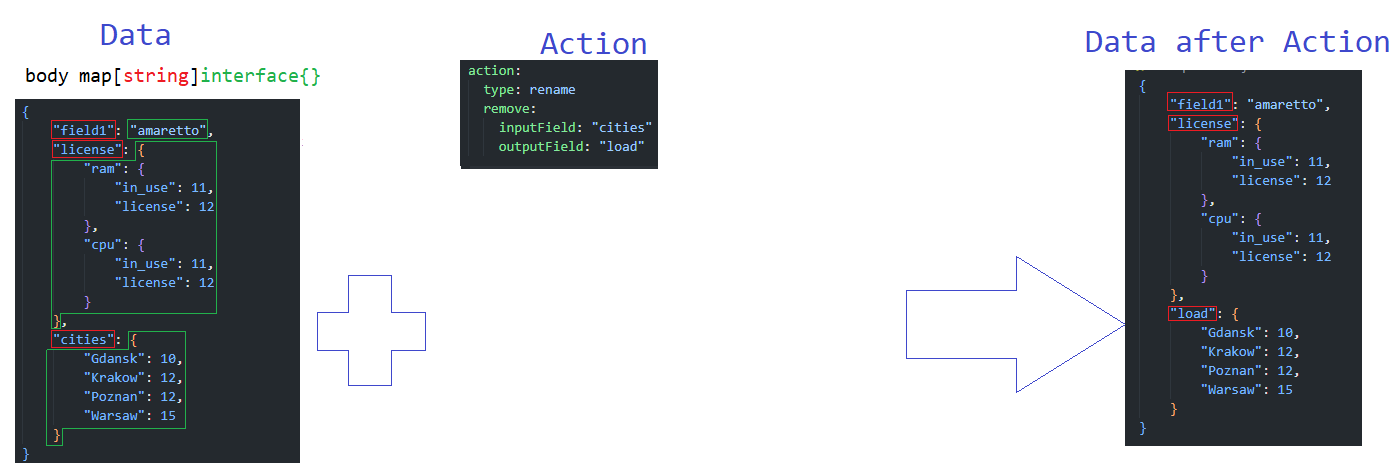
\includegraphics[width=1\linewidth]{a6-duplicate.png}
    \caption{Przykład modyfikacji danych przez akcje Duplicate}\label{fig:a6-duplicate}
\end{figure}
\subsubsection{Insert}
